% **************************************************************************** %
%                                                                              %
%                                                     ::::::::  :::::::::      %
%    sec_intro.tex                                      :+:      :+:    :+:    %
%                                                    +:+        +:+    +:+     %
%    By: A. Campo <andoitzcp@gmail.com>              +#+        +#++:++#+      %
%                                                    +#+        +#+            %
%    Created: 2022/11/18 22:55:54 by A. Campo        #+#    #+# #+#            %
%    Updated: 2023/02/10 03:54:56 by acampo-p         ###   ########.fr        %
%                                                                              %
% **************************************************************************** %

\section{INTRODUCCIÓN}\label{sec:intro}

El sector de la automoción,
engloba una gran variedad de industria y servicios dedicados a servirla.
Se estima que la aportación económica total de las actividades relacionadas,
en este sector, asciende a un 11\% del PIB,
lo que la convierte en la industria manufacturera que mas ingresos aporta
después  del 18,8\% del PIB que posee la industria agroalimentaria española
(Díaz y Montorriol Garriga, 2021).

En este sector, el vehículo de propulsión autónoma,
es generalmente utilizado tanto por los servicios de transporte a pasajero,
como por los servicios logísticos dedicados al transporte de mercancías.
Entre los componentes que forman el vehículo autónomo,
se encuentran las cubiertas o neumáticos,
los cuales se comportan como enlace entre el vehículo y el pavimento.
Este nexo permite una transmisión eficiente
de la energía producida por el motor de combustión interna,
y a su vez, sus propiedades elásticas atenúan las irregularidades de la vía.

La industria manufacturera de cubiertas,
ha mantenido un incremento sostenido en su producción en los últimos años,
como puede observarse en la Figura \ref{fig:1_global_prod_evo}.
El mercado de neumáticos es liderado por dos empresas: Bridgestone y Michelin
\citep{rodgers2020tire}.
Las demás empresas compiten entre ellas
a un magnitud inferior a los lideres del sector,
como se aprecia en la Figura \ref{fig:1_brand_revenue}.

\begin{figure}[h]
	\begin{center}
		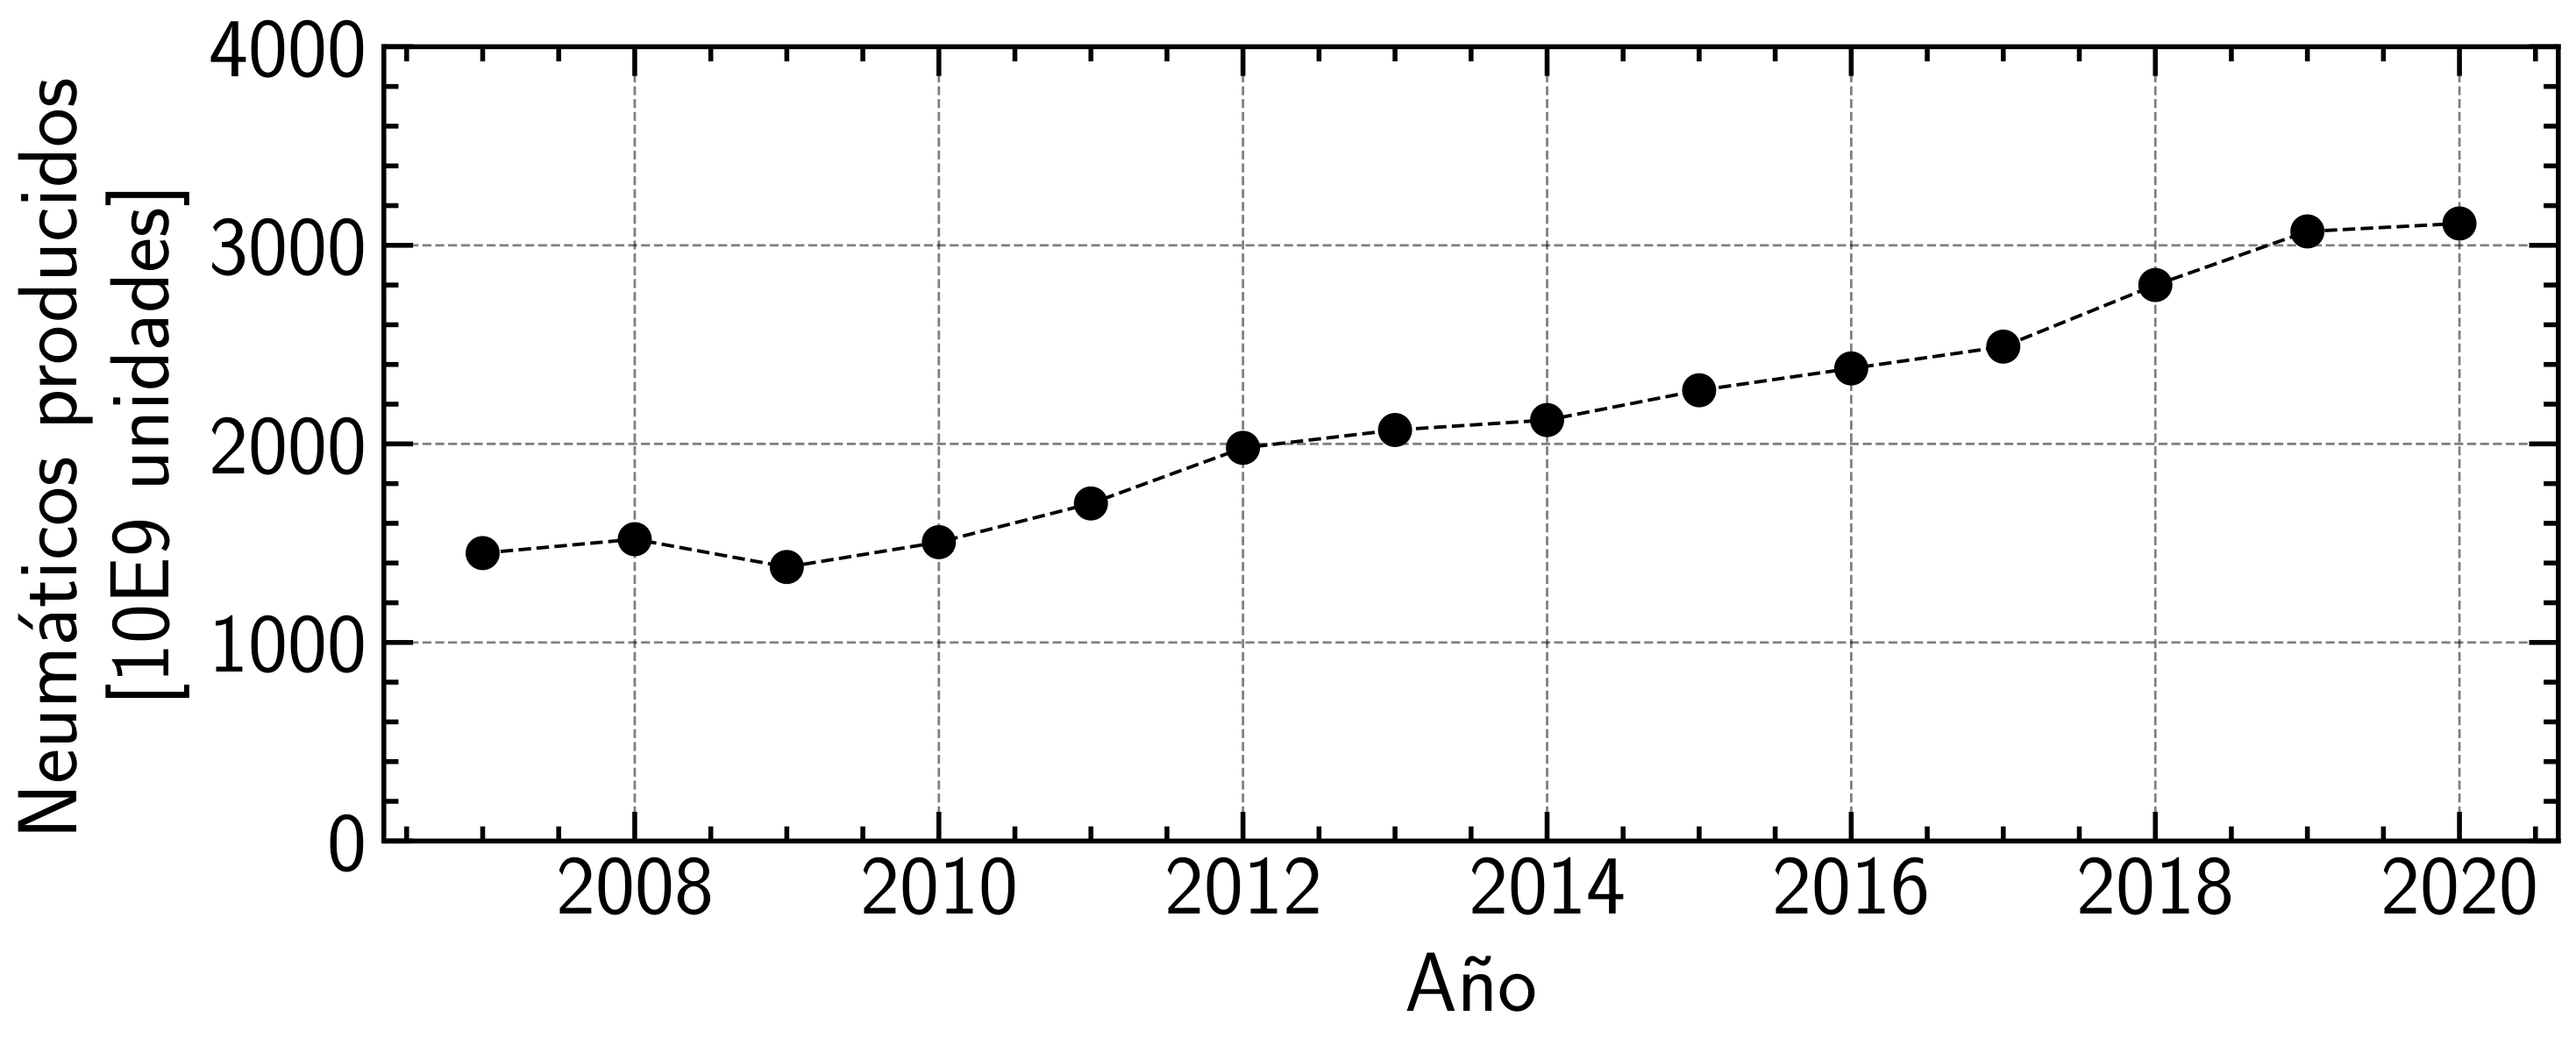
\includegraphics[width=\textwidth]{fig/1_global_prod_evo.PNG}
	\end{center}
	\caption{Evolución de la producción mundial de cubiertas \citep{rodgers2020tire}.}
	\label{fig:1_global_prod_evo}
\end{figure}

 \begin{figure}[h]
	\begin{center}
		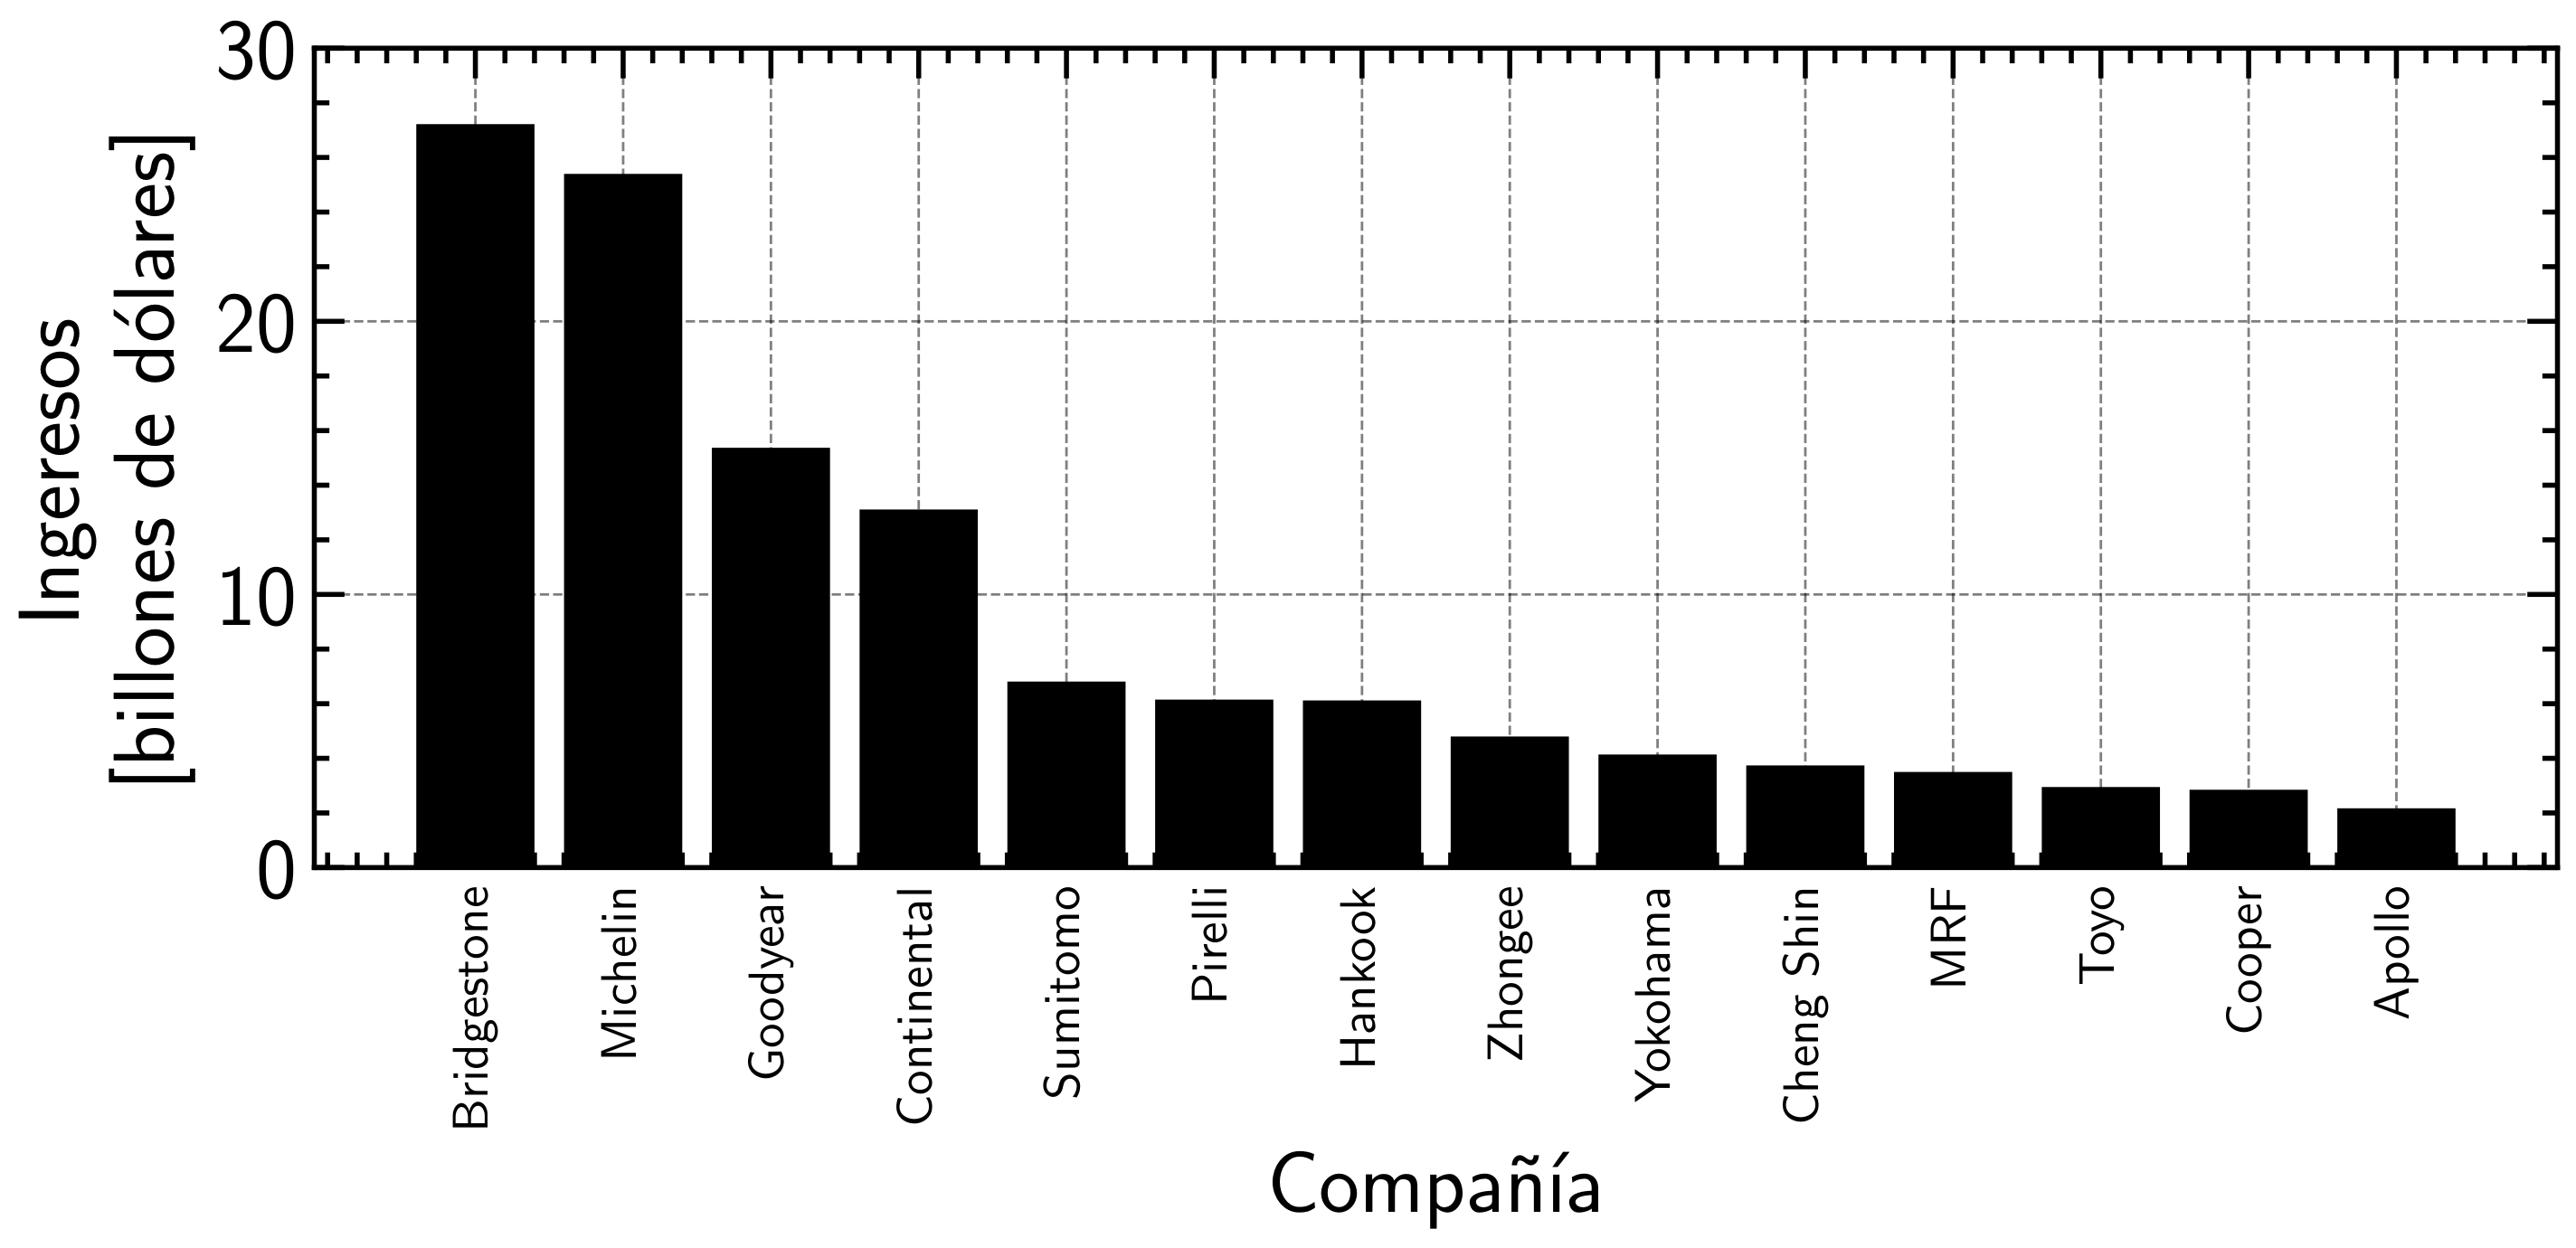
\includegraphics[width=\textwidth]{fig/1_brand.revenue.PNG}
	\end{center}
	\caption{Ingresos de los fabricantes de neumáticos más relevantes en 2019 \citep{rodgers2020tire}.}
	\label{fig:1_brand_revenue}
\end{figure}

La elevada competitividad característica del mercado,
sumada a la emergente comercialización de producto asiático,
incentiva a las establecidas multinacionales, a tomar un enfoque innovativo,
con la intención de mantener su liderazgo \citep{chicu2020current}.
El esfuerzo invertido en innovación,
por una parte, intenta alcanzar sus objetivos
mediante el rediseño y la mejora del producto.
Mientras que por la otra,
trata de optimizar sus procesos y reducir desperdicios,
mediante la automatización y el uso inteligente de los recursos disponibles.

A la hora de implementar mejoras, ya sea a un producto o a un proceso,
la monitorización de los resultados se vuelve esencial.
El producto o proceso experimental debe satisfacer las expectativas del cliente,y a su vez, cumplimentar la legislación vigente,
como los estándares de calidad y medio ambiente.
La monitorización de estas mejoras implica un coste elevado,
a nivel temporal y económico, ya que estas deben ser puestas a prueba.
En el caso del producto, su industrialización,
supone reservar recursos que podrían ser destinados a la producción regular.
Desde la materia prima utilizada
en la elaboración de estos productos experimentales,
a través de cada maquina ocupada para transformarlo,
hasta llegar a el laboratorio de calidad,
donde se realizan ensayos para otorgar feedback a el cliente.

En las empresas de neumáticos, el laboratorio de Calidad del Producto (LCP),
es el encargado de llevar a cabo los ensayos relevantes
para asegurar la conformidad de la producción.
A diario se cerciora de que los neumáticos manufacturados dentro de la planta
cumpla con los estándares de calidad definidos por la compañía.
El laboratorio logra asegurar la calidad del producto,
mediante un control estadístico de las muestras
elegidas al azar por cada gamma de producto.
Paralelamente, una fracción de los recursos disponibles,
es demandada por los proyectos de industrialización.
Obligando al departamento a equilibrar ambas necesidades.

En un entorno con recursos limitados,
donde la demanda no cesa de incrementar,
es cuestión de tiempo que los recursos se agoten
y la capacidad de el laboratorio se vea sobrepasada.
Para hacer frente a esta situación,
y poder mantener el esencial ritmo
marcado por los estándares de control de calidad e industrialización,
debe realizarse un escalado de los recursos del LCP.
A fin de que esta expansión, de este sistema complejo,
se realice de la manera optima,
debe realizarse un estudio de el impacto
de las inversiones que podrían realizarse, en la capacidad del LCP.
Debido a que experimentar con el sistema real,
y desarrollar una solución analítica no es factible,
se ha propuesto el uso de la simulación.
Dentro de los tipos de simulación, existen varias alternativas.

\begin{itemize}
	\item Simulación Monte Carlo: Este tipo de simulaciones toma el nombre
		del famoso casino ubicado en Mónaco.
		Este tipo de simulación se caracteriza por desencadenar un evento
		una y otra vez con el fin de obtener los resultados esperados.
		Suele ser utilizado con el fin de aproximar
		expresiones matemáticas complejas.
		Este método puede ser usado, por ejemplo,
		para determinar la probabilidad de que
		un dado obtenga como resultado
		al menos un 5 en 4 de cada diez tiradas.
		Siendo esta aproximación tan sencilla,
		resulta fácil de implementar,
		aunque el análisis de los resultados puede verse limitado
		debido a su sencillez.
	\item Cadena de Markov: La cadena de Markov,
		es un modelo estocástico que describe
		una secuencia de posibles eventos,
		en los que la probabilidad de cada evento
		depende únicamente del estado del evento anterior.
		Mediante este modelo, se pueden representar
		de manera sencilla sistemas estadísticos complejos.
		Mientras que este tipo de simulación
		es comúnmente utilizado en la cuántica,
		los procesos industriales presentan
		una gran interdependencia entre procesos,
		reduciendo la variedad de procesos que pueden
		ser efectivamente modelados por este tipo de simulación.
	\item Simulación de Eventos Discretos (DES):
		Las DES toman el enfoque de representar sistemas reales
		mediante la ejecución y concatenación
		de procesos en un entorno virtual.
		Esta representación computacional, se asemeja al sistema real.
		La DES ha demostrado su capacidad de resolver
		problemas de optimización en sistemas estocásticos.
		Como menciona el \citep{allen2011introduction},
		su versatilidad ha sido demostrada en numerosos ámbitos,como
		aplicaciones militares,
		sistemas sanitarios,
		problemas logísticos
		y optimización de procesos de manufacturación.
\end{itemize}

\subsection{EL LABORATORIO DE CALIDAD DEL \newline PRODUCTO}

A lo largo del proceso de fabricación de una cubierta,
son varios los estándares de calidad que debe cumplir el producto
para que pueda ser vendido en los distintos mercados a nivel global.
Desde la composición química de las materias primas usadas,
hasta las propiedades físicas del producto finalizado,
la certificación de que el producto se halla dentro de los limites especificados,
asegura un producto de calidad.

En el proceso final de control de calidad
que se lleva a cabo en un laboratorio de evaluación del producto,
estos son los ensayos principales.

\begin{itemize}
	\item Ensayos \textit{Endurance}
	\item Ensayos \textit{Rolling Resistance}
	\item Ensayos dimensionales
\end{itemize}

En el LCP,
son dos clientes internos los que comparten los recursos disponibles.
Por una parte, se encuentran los procesos de conformidad de la producción (CP),
encargados de aseguramiento de la calidad
de el producto destinado a la venta a clientes
Por otra parte, se encuentran los procesos de desarrollo de nuevos productos,
o el departamento de industrialización (IND),
encargados de desarrollar nuevas lineas del producto,
y optimizar los procesos de producción
mediante cambios controlados que suceden en grupos reducidos.
Finalmente, se reciben solicitudes de ensayo de ajenos al laboratorio,
que simularían los encargos particulares que recibe el laboratorio,
a través de otras vías (EXT).
Para este caso, en el LCP, se ha estimado que,
estas 3 fuentes de muestras de ensayo
suman la cantidad descrita en la tabla~\ref{tab:2_tbl_actual_demand}.
La cual esta cerca, de los límites de capacidad teóricos
para un laboratorio con el equipamiento descrito en
las tablas~\ref{tab:3_tbl_sim_det} y~\ref{tab:3_tbl_rsrc}.
Las perspectivas de futuro, prevén que el incremento
de la actividad en el mercado continúe,
por lo que el LCP deberá afrontar una demanda superior a su capacidad estimada.

\begin{table}
	\centering
	\caption{Suma de la demanda estimada de ensayos por tipo de ensayo.}
	\documentclass[varwidth=\maxdimen]{standalone}
\usepackage[utf8]{inputenc}
\usepackage[spanish]{babel}
\usepackage{booktabs}

\begin{document}

\begin{tabular}{ l c }
	\toprule
	Ensayo & Demanda (unds.) \\
	\midrule
	Endurance	& 280 \\
	Rolling		& 760 \\
	Dimensional	& 140 \\
	\bottomrule
\end{tabular}

\end{document}

	\label{tab:2_tbl_actual_demand}
\end{table}

El flujo de los procesos llevados a cabo en el laboratorio,
se representa en la Figura~\ref{fig:2_fc_lep_diagram}.

\begin{figure}
	\begin{center}
		\includestandalone{fig/2_fc_lep_diagram}
	\end{center}
	\caption{Diagrama de flujo de los procesos llevados a capo en el Laboratorio de Evaluación del Producto.}
	\label{fig:2_fc_lep_diagram}
\end{figure}

\subsubsection{Ensayos Endurance}
Estos ensayos someten a las cubiertas a unas condiciones particularmente extremas
que no se llegan a alcanzar dentro del margen de uso habitual
para el que están diseñadas.
El ensayo consiste en hacer rodar el objeto de ensayo
durante un periodo aproximado de 72 horas a una temperatura constante de 40 ºC,
aumentando la carga en pasos discretos a lo largo del test.

El laboratorio dispone de 4 maquinas
similares a la que aparece en la Figura~\ref{fig:2_endurance_machine},
cada una de ellas teniendo la capacidad de montar hasta 2 cubiertas.

El ensayo se comunica como exitoso
si el objeto de ensayo no ha sufrido deformaciones
antes de el tiempo específico para cada producto.
Una vez finalizado el test, 2 secciones se cortan y se pulen 
por un operario y se almacenan para la elaboración del informe. 

\begin{figure}
	\begin{center}
		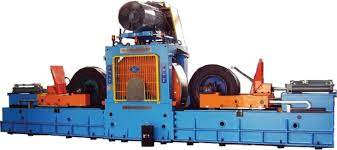
\includegraphics[width=\textwidth]{fig/2_endurance_machine}
	\end{center}
	\caption{Maquina utilizada en los ensayos Endurance}
	\label{fig:2_endurance_machine}
\end{figure}

\subsubsection{Ensayos Rolling Resistance}
El objetivo de este ensayo es determinar el consumo energético
de la cubierta debido a la fricción causada mientras rueda.
La maquina que aparece en la Figura~\ref{fig:2_rr_machine} mide la resistencia que ofrece
el objeto de ensayo a 25 ºC.
La duración media del ensayo es de unas 3 horas.
La particularidad de este ensayo consiste en que
el resultado es sensible a la presión de inflado y temperatura de la sala.
Debido a esto, la mayor parte del ensayo
consiste en asegurar que la cubierta alcance el estado estable,
siendo los últimos 10 minutos el tiempo en el que
ocurre la medición de la resistencia a la rodadura.

\begin{figure}
	\begin{center}
		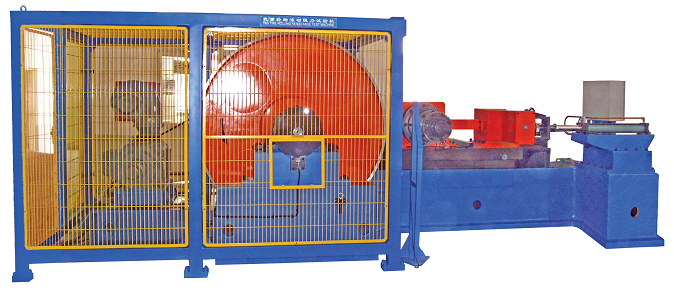
\includegraphics[width=\textwidth]{fig/2_rr_machine}
	\end{center}
	\caption{Maquina utilizada en los ensayos Rolling Resistance}
	\label{fig:2_rr_machine}
\end{figure}

El laboratorio dispone de una maquina capaz de realizar estos ensayos.
Dentro de la sala de la maquina, hay espacio para almacenar cubiertas
para que estén acondicionadas a la hora de preparar el siguiente ensayo.

\subsubsection{Análisis dimensional}
El objetivo de este ensayo es verificar que
tanto las dimensiones generales de la cubierta,
como sus componentes internos
quedan dentro de la tolerancia de las especificaciones.

Para ello, el laboratorio dispone de 2 técnicos adicionales
que se dedican únicamente a llevar a cabo estos análisis.


\subsection{OBJETIVOS}\label{sec_obj}
El objetivo principal de este trabajo
es proveer a la planta hipotética de cubiertas
con la información necesaria para la optima expansión del LCP.
Este trabajo se limitara a analizar los distintos escenarios investigados,
ofreciendo métricas e información cualitativa
sobre las distintas posibilidades,
para finalmente decantarse por la mejor opción.

Para lograr el objetivo final se deberán completar los siguientes subobjetivos:

\begin{itemize}
	\item Modelar los procesos del LCP
		de acuerdo a los fundamentos de una DES,
		obteniendo un modelo ajustado a la realidad.
	\item Definir las variables independientes del proceso,
		que posteriormente serán usadas en la simulación.
	\item Estimar el tiempo de ciclo de cada proceso,
		a través de la asignación de
		distribuciones ajustadas a cada subproceso.
	\item Definir las variables dependientes
		que otorgara el sistema a la salida.
	\item Desarrollar un programa de simulación en el entorno de Python
		mediante el uso de la librería Simpy.
		Dicha simulación, sera capaz de emular
		los distintos escenarios propuestos durante el desarrollo.
	\item Proponer una alternativa de la distribución de los recursos actuales
		para asegurar la capacidad del LCP cuando en el futuro aumente la
		demanda de ensayos.
\end{itemize}
